These are some representations of how the mobile application should look like.\\ 
\subsection{Mockups}
In this section some concept Mockups that were used to then develop the first iteration of the application are shown, it should be noted that the finished product must follow the concept of these designs and not use the actual graphical elements here showcased, but a professional artist should be instead hired to design the interface given these guidelines.

\begin{figure}[h]
\centering
\begin{subfigure}{.5\textwidth}
  \centering
  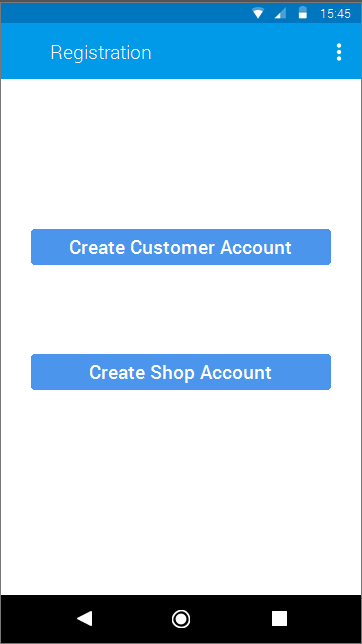
\includegraphics[height=.4\textheight, keepaspectratio=true]{Img/Mockup_Registration}
  \caption{User type choice}
\end{subfigure}%
\begin{subfigure}{.5\textwidth}
  \centering
  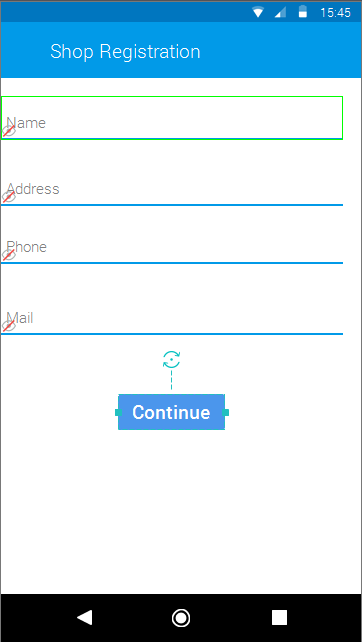
\includegraphics[height=.4\textheight, keepaspectratio=true]{Img/Mockup_RegistrationShop1}
  \caption{Shop registration}
\end{subfigure}
\caption{Login on the left (a) and first step of Shop registration on the right (b)}
\end{figure}

\begin{figure}[h]
\centering
\begin{subfigure}{.5\textwidth}
  \centering
  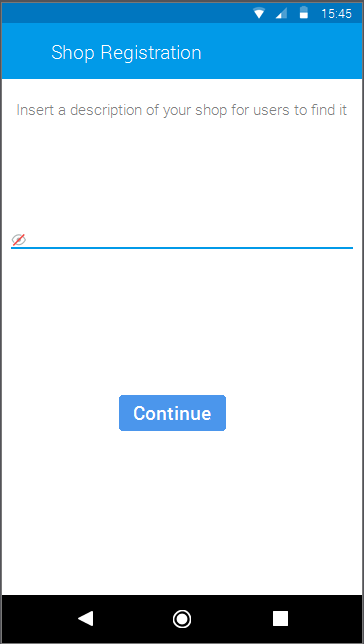
\includegraphics[height=.4\textheight, keepaspectratio=true]{Img/Mockup_RegistrationShop2}
  \caption{Shop description request}
\end{subfigure}%
\begin{subfigure}{.5\textwidth}
  \centering
  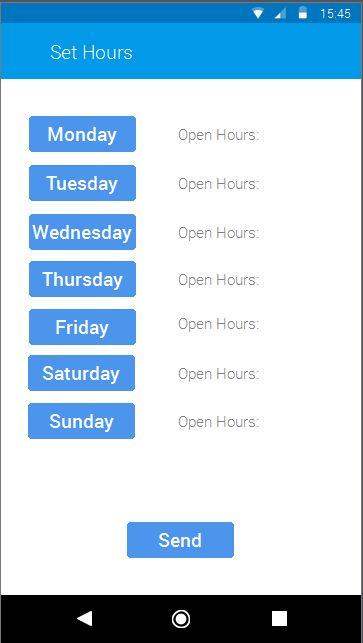
\includegraphics[height=.4\textheight, keepaspectratio=true]{Img/Mockup_RegistrationShop3}
  \caption{Shop hours request}
\end{subfigure}
\caption{Second page for shop registration (a) and third one(b)}
\end{figure}

\begin{figure}[h]
\centering
\begin{subfigure}{.5\textwidth}
  \centering
  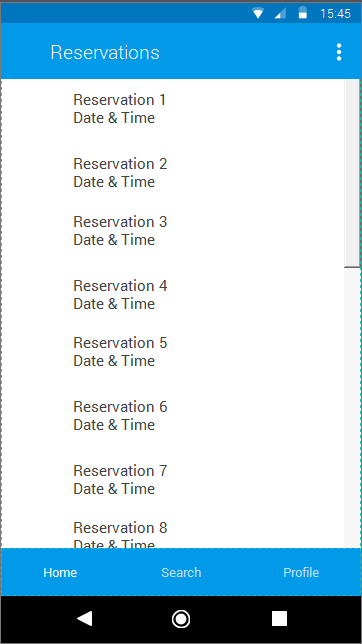
\includegraphics[height=.4\textheight, keepaspectratio=true]{Img/Mockup_Customer_Home}
  \caption{Customer Home}
\end{subfigure}%
\begin{subfigure}{.5\textwidth}
  \centering
  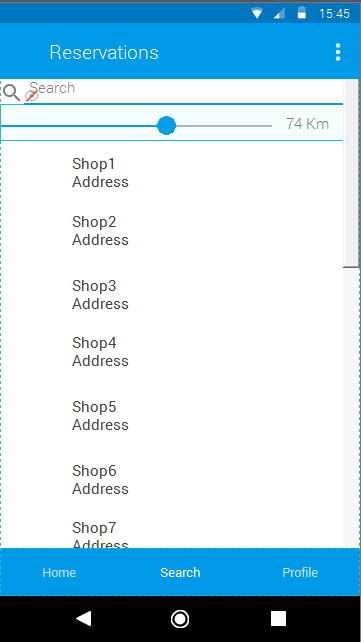
\includegraphics[height=.4\textheight, keepaspectratio=true]{Img/Mockup_Customer_Search}
  \caption{Customer Search}
\end{subfigure}
\caption{The customer's home page (a) and the search screen (b)}
\end{figure}
\clearpage
\subsection{Application Screenshots}
Here are instead shown the screenshots of the implementation of the application from the emulator. Some pages are not shown since they would look the same as others (for example editing a shop's information opens the same screens of the registration with the fields already inserted).

\begin{figure}[h]
\centering
\begin{subfigure}{.5\textwidth}
  \centering
  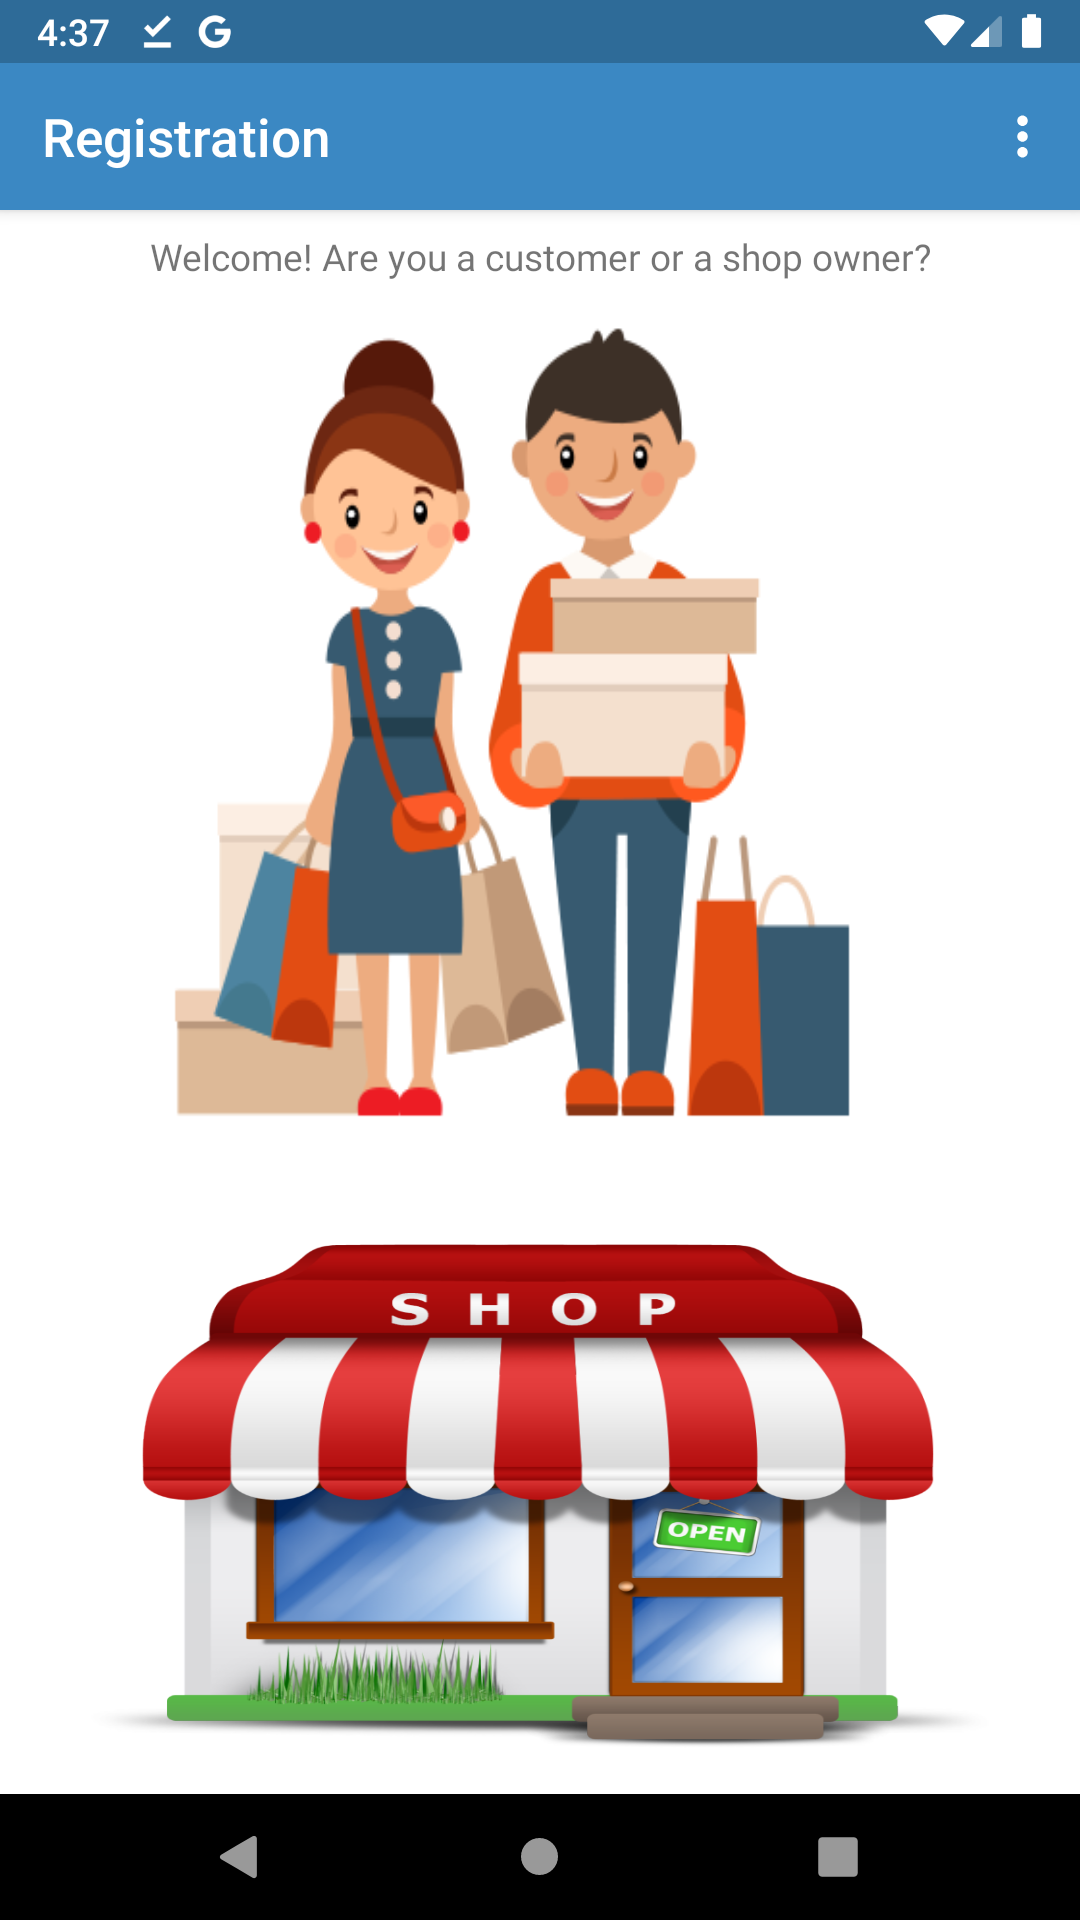
\includegraphics[height=.4\textheight, keepaspectratio=true]{Img/Screens/Registration_Home}
  \caption{Registration Home}
\end{subfigure}%
\begin{subfigure}{.5\textwidth}
  \centering
  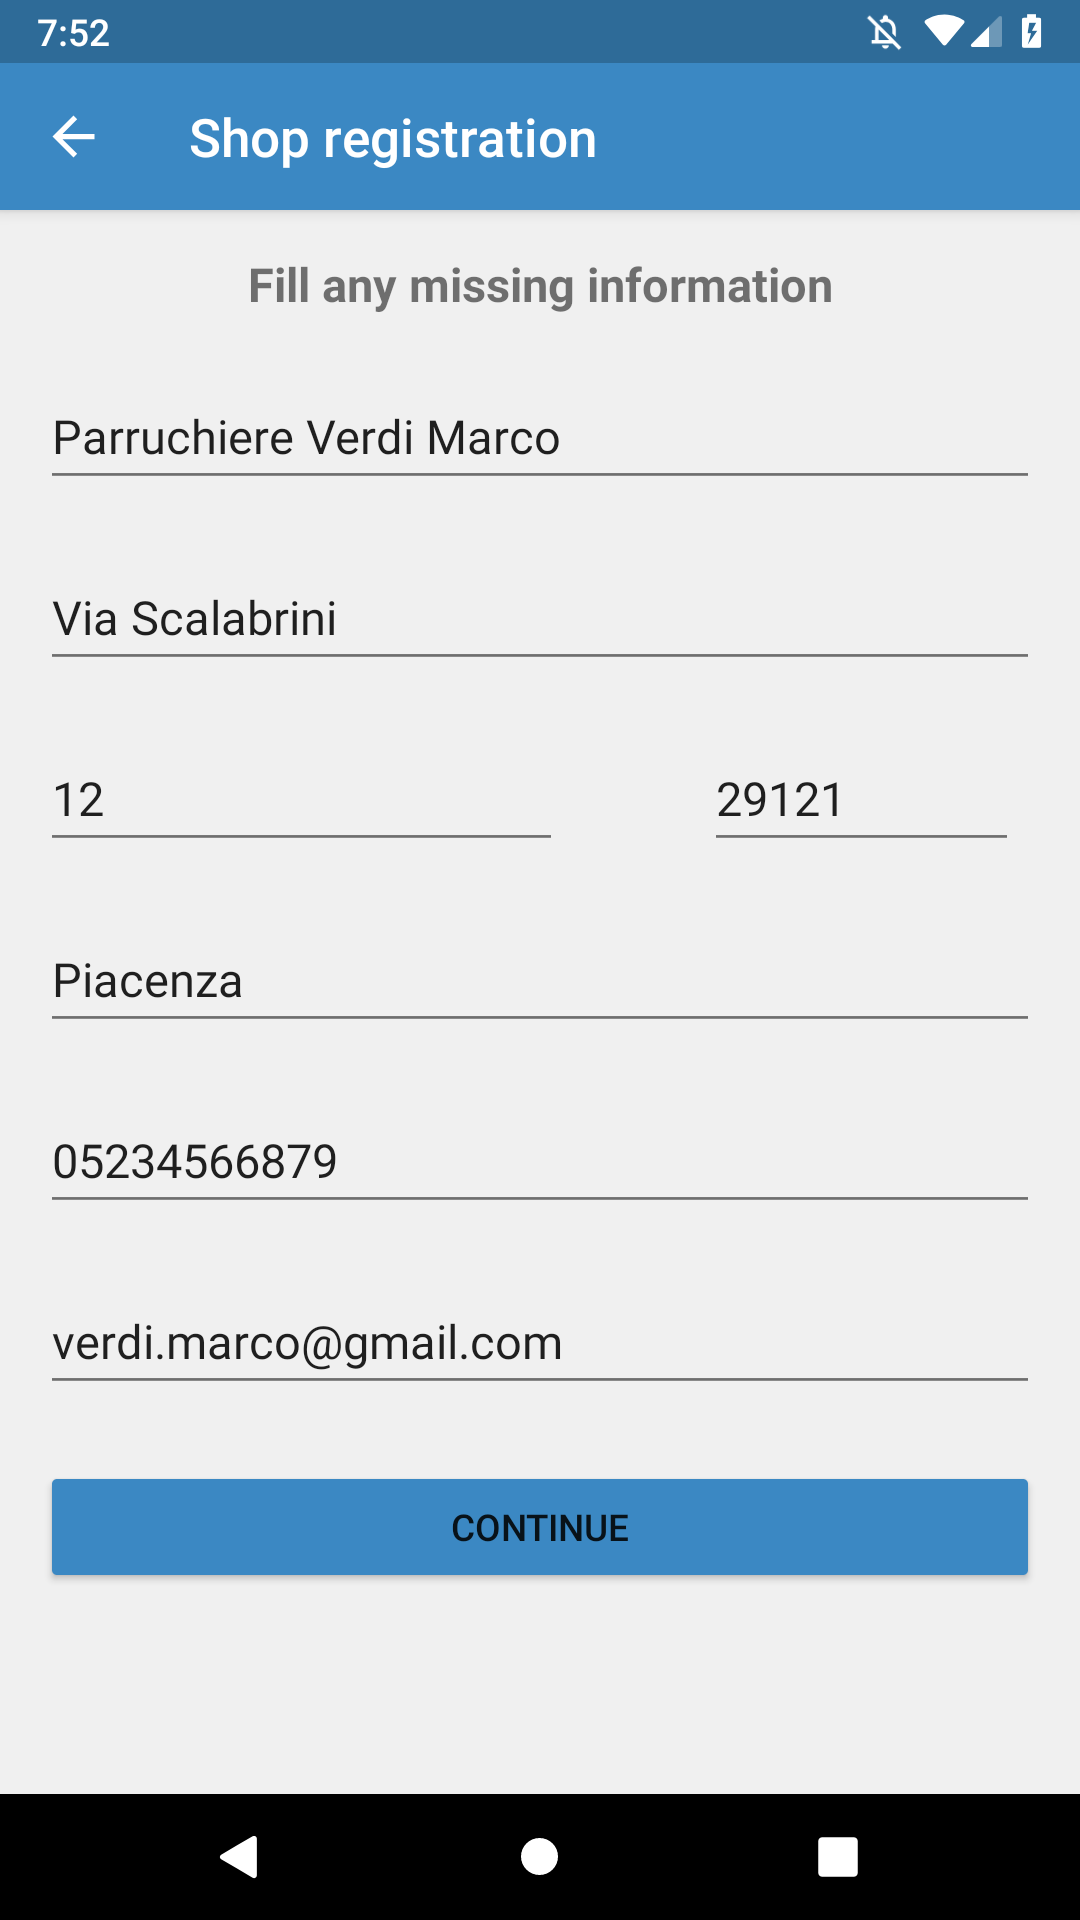
\includegraphics[height=.4\textheight, keepaspectratio=true]{Img/Screens/Registration_Shop1}
  \caption{First shop registration page}
\end{subfigure}
\caption{Registration home on the left(a) first of the two registration pages for the shop on the right(b)}
\end{figure}

\begin{figure}[h]
\centering
\begin{subfigure}{.5\textwidth}
  \centering
  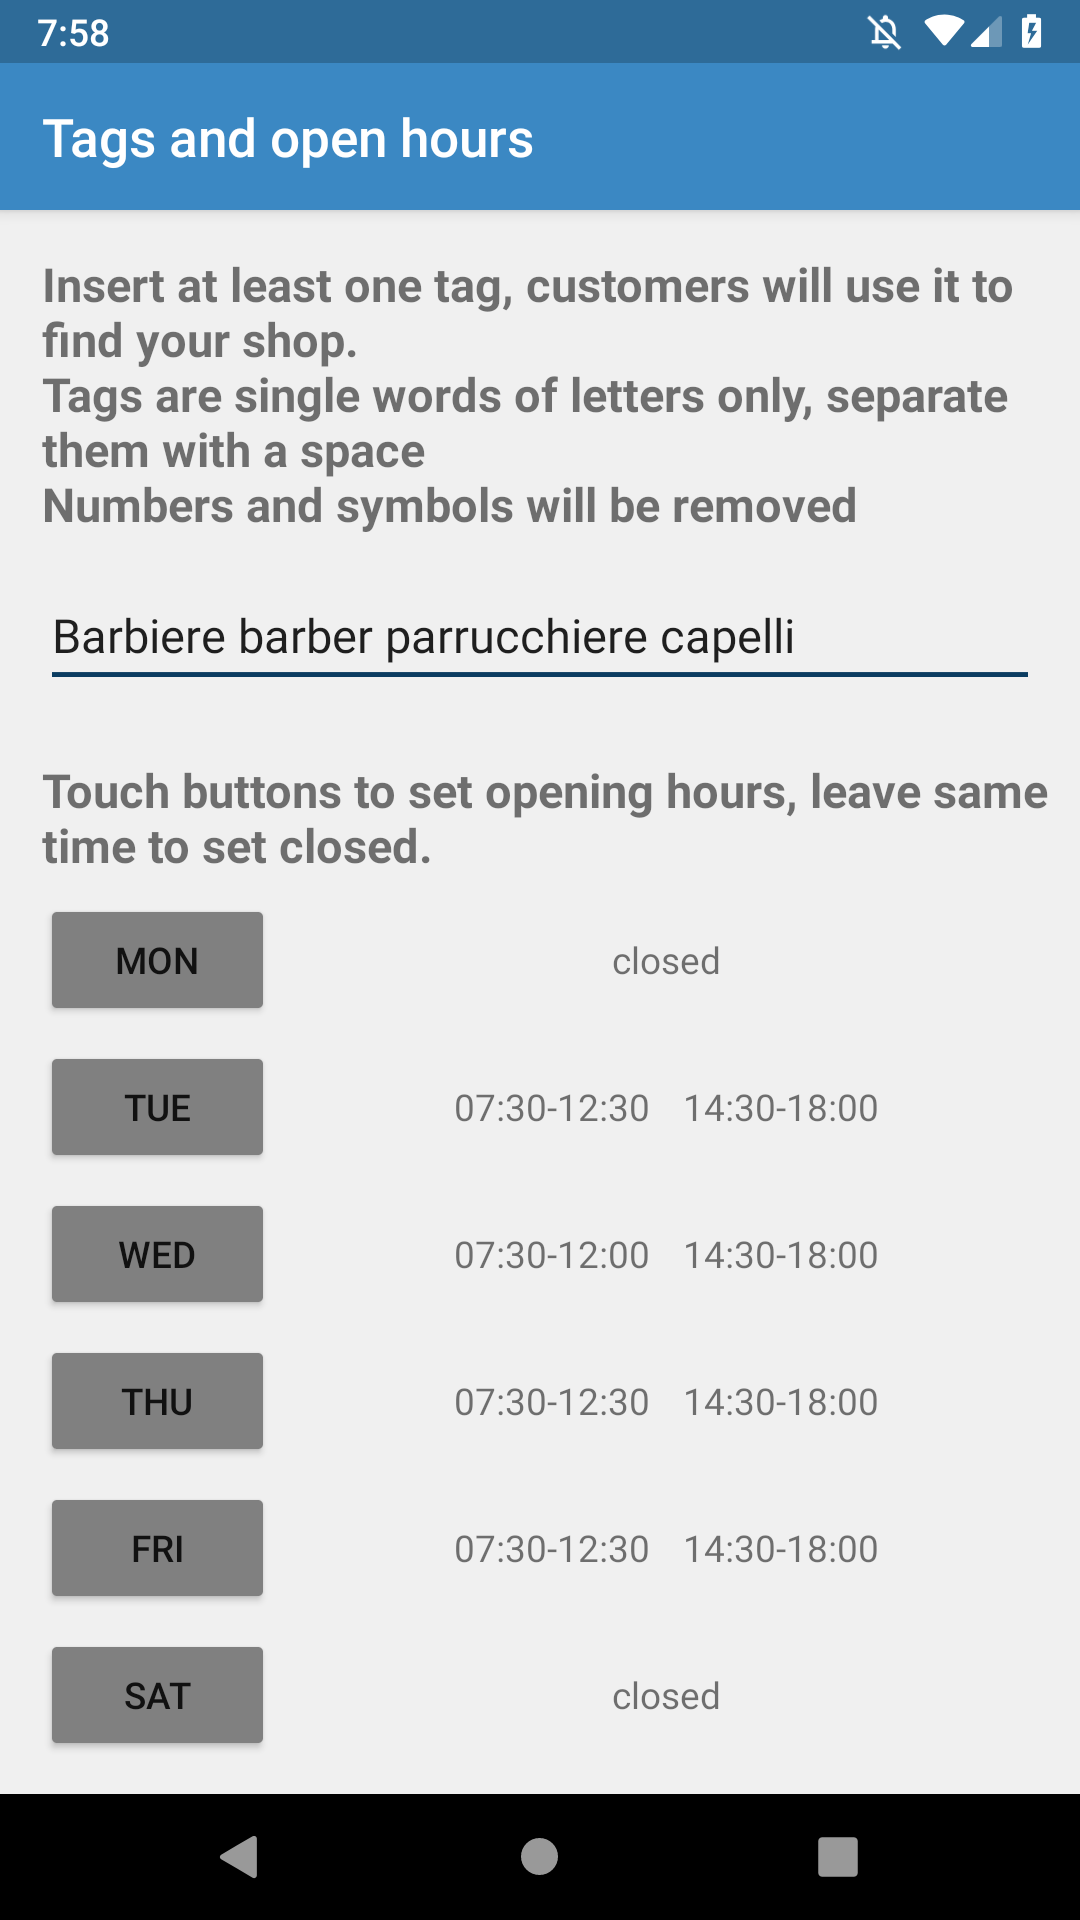
\includegraphics[height=.4\textheight, keepaspectratio=true]{Img/Screens/Registration_Shop2}
  \caption{Insertion of tags and selection of opening hours}
\end{subfigure}%
\begin{subfigure}{.5\textwidth}
  \centering
  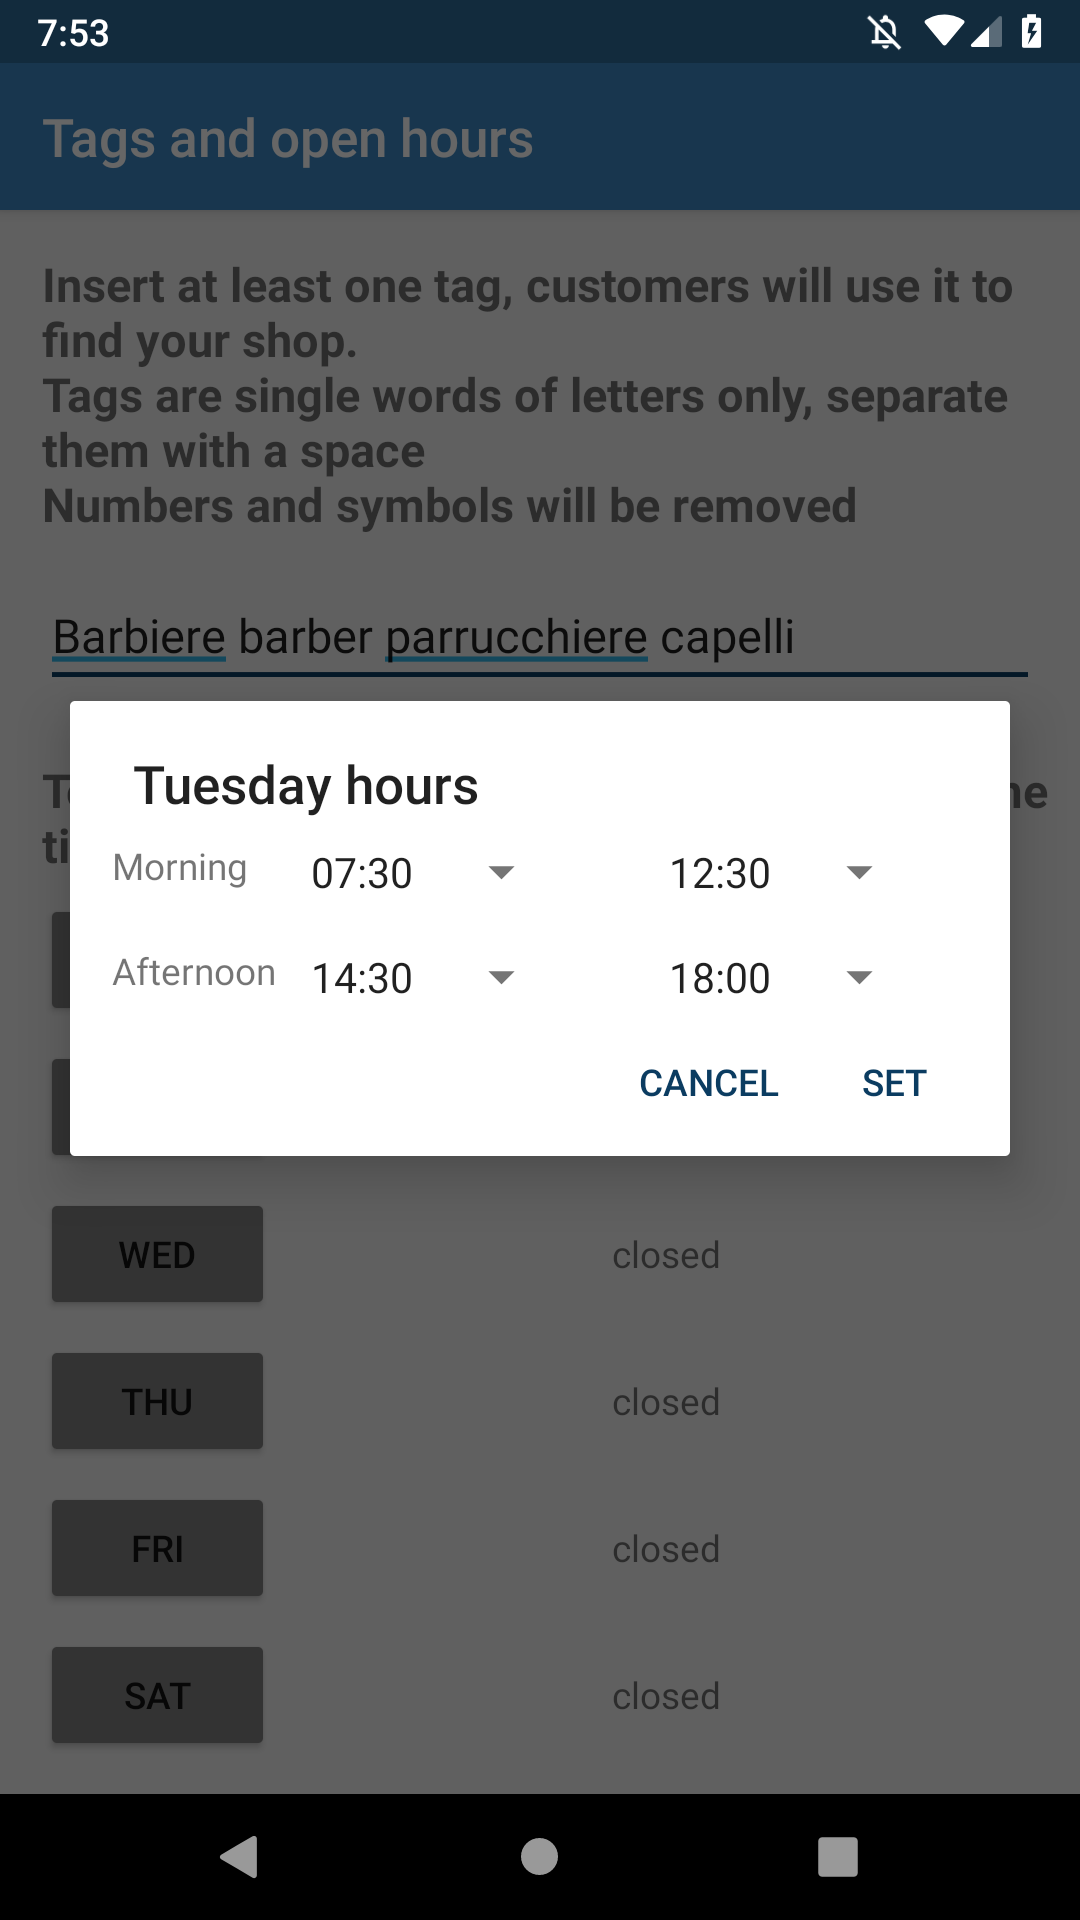
\includegraphics[height=.4\textheight, keepaspectratio=true]{Img/Screens/Registration_Shop3}
  \caption{Opening hours detail}
\end{subfigure}
\caption{Page for inserting tags and hours (a) with detail of the alert shown to pick times(b).\\Last buttons are below the view.}
\end{figure}

\begin{figure}[h]
\centering
\begin{subfigure}{.5\textwidth}
  \centering
  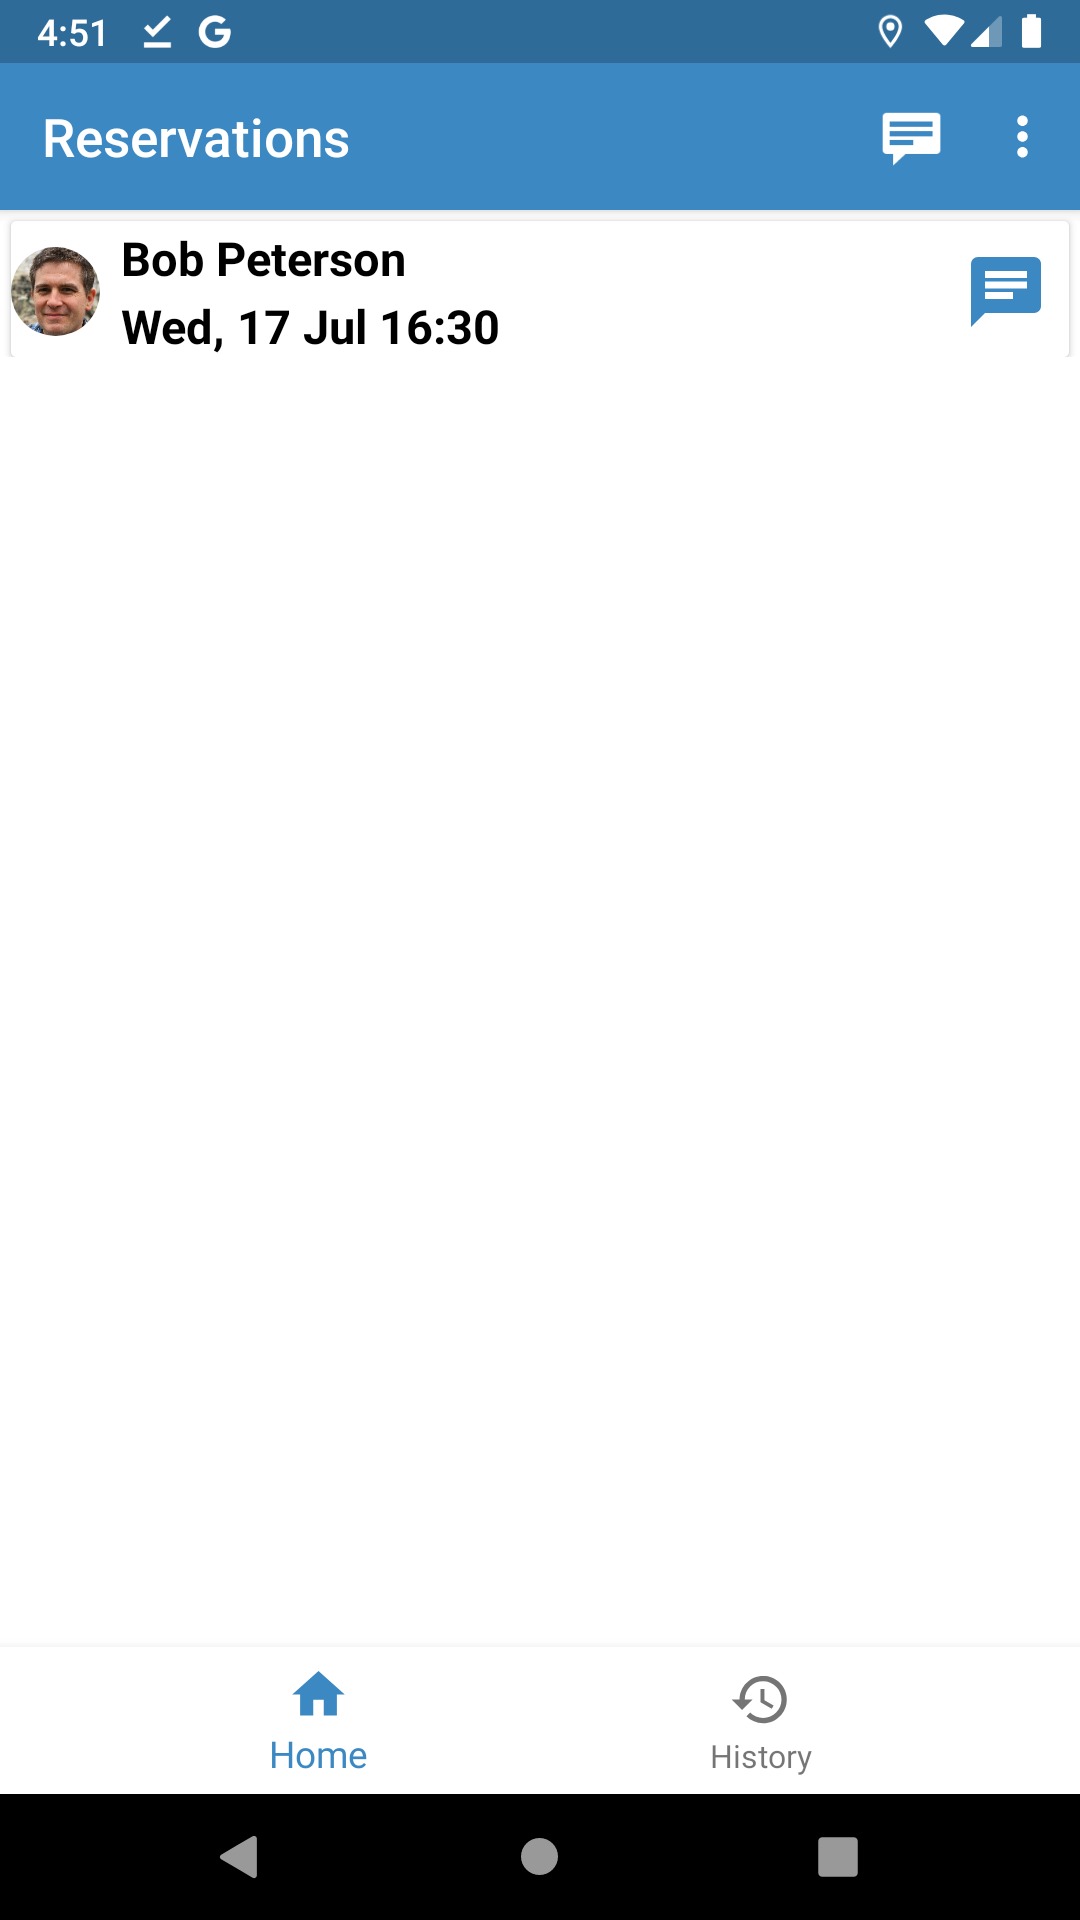
\includegraphics[height=.4\textheight, keepaspectratio=true]{Img/Screens/Shop_Home}
  \caption{Shop's home page}
\end{subfigure}%
\begin{subfigure}{.5\textwidth}
  \centering
  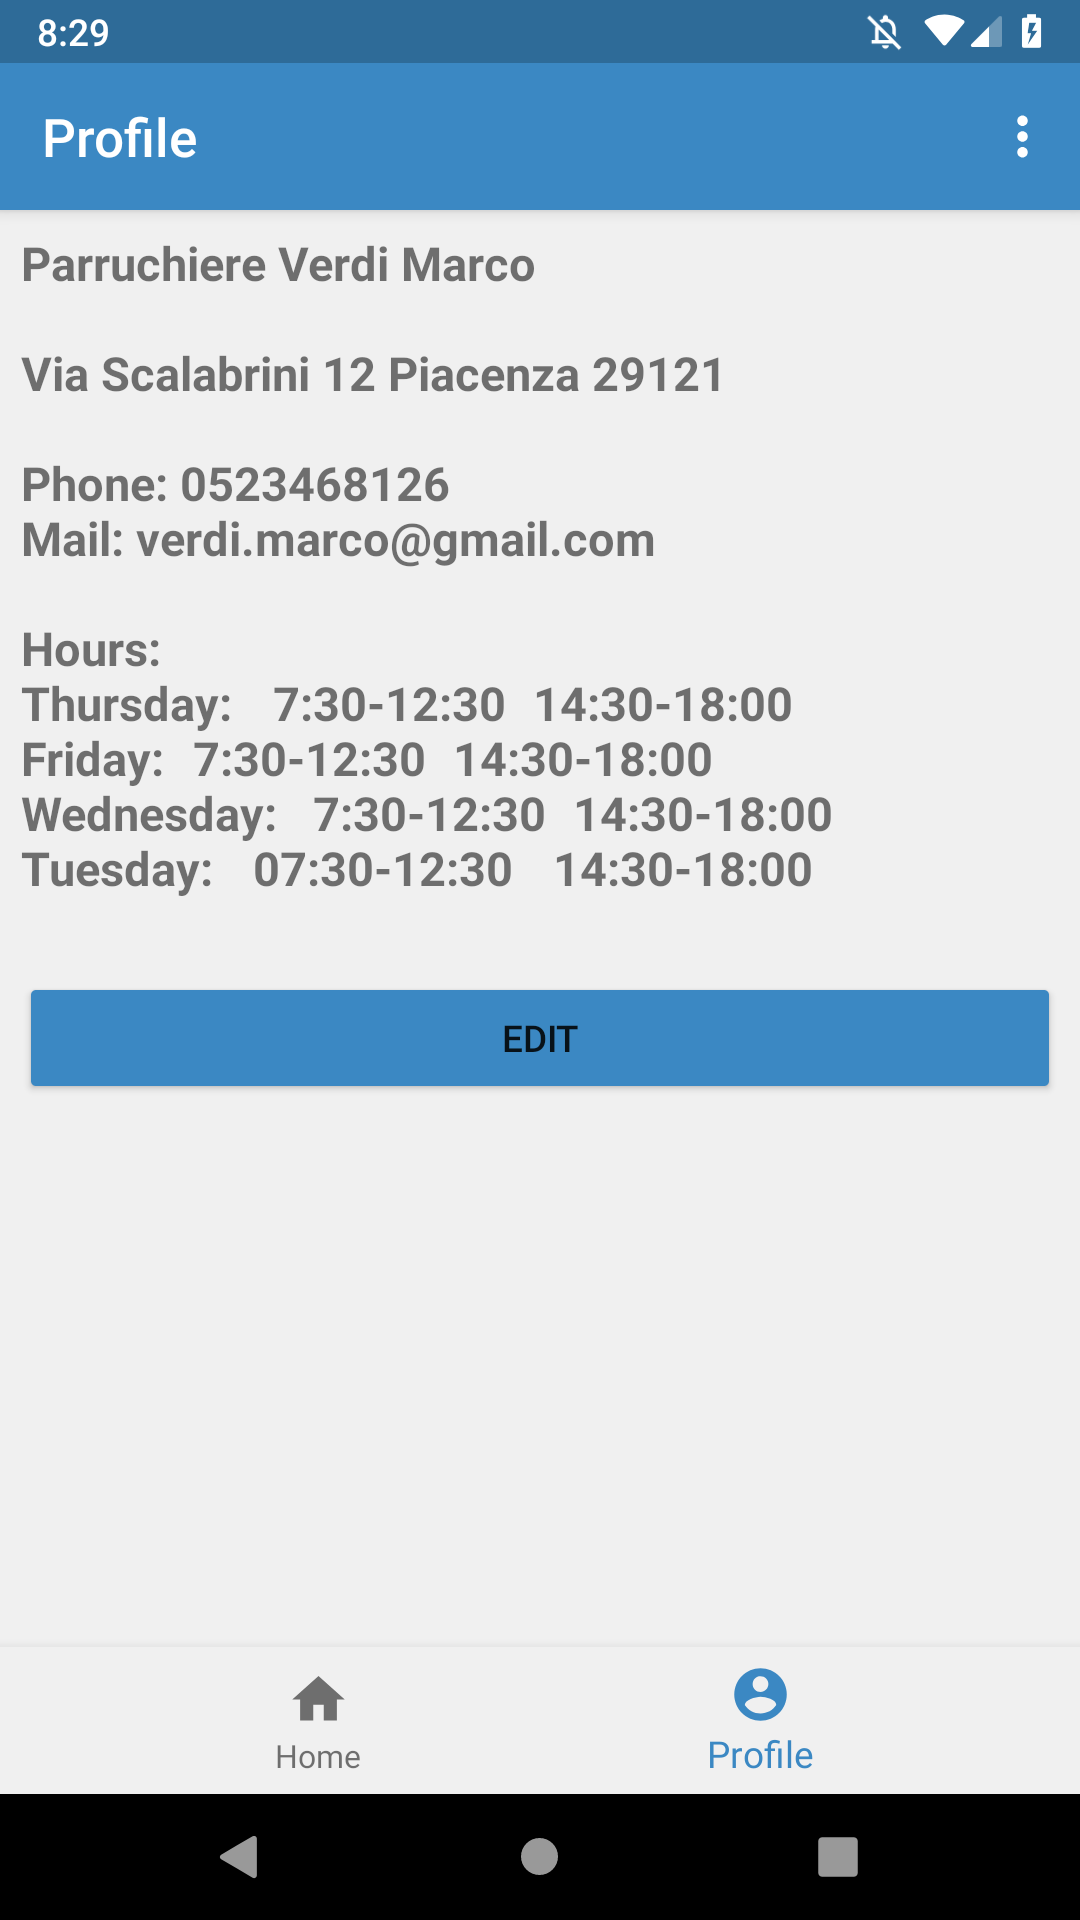
\includegraphics[height=.4\textheight, keepaspectratio=true]{Img/Screens/Shop_Profile}
  \caption{Shop's profile}
\end{subfigure}
\caption{Shop home page with next reservations (a) and shop profile recap with button to edit info(b).}
\end{figure}

\begin{figure}[h]
\centering
\begin{subfigure}{.5\textwidth}
  \centering
  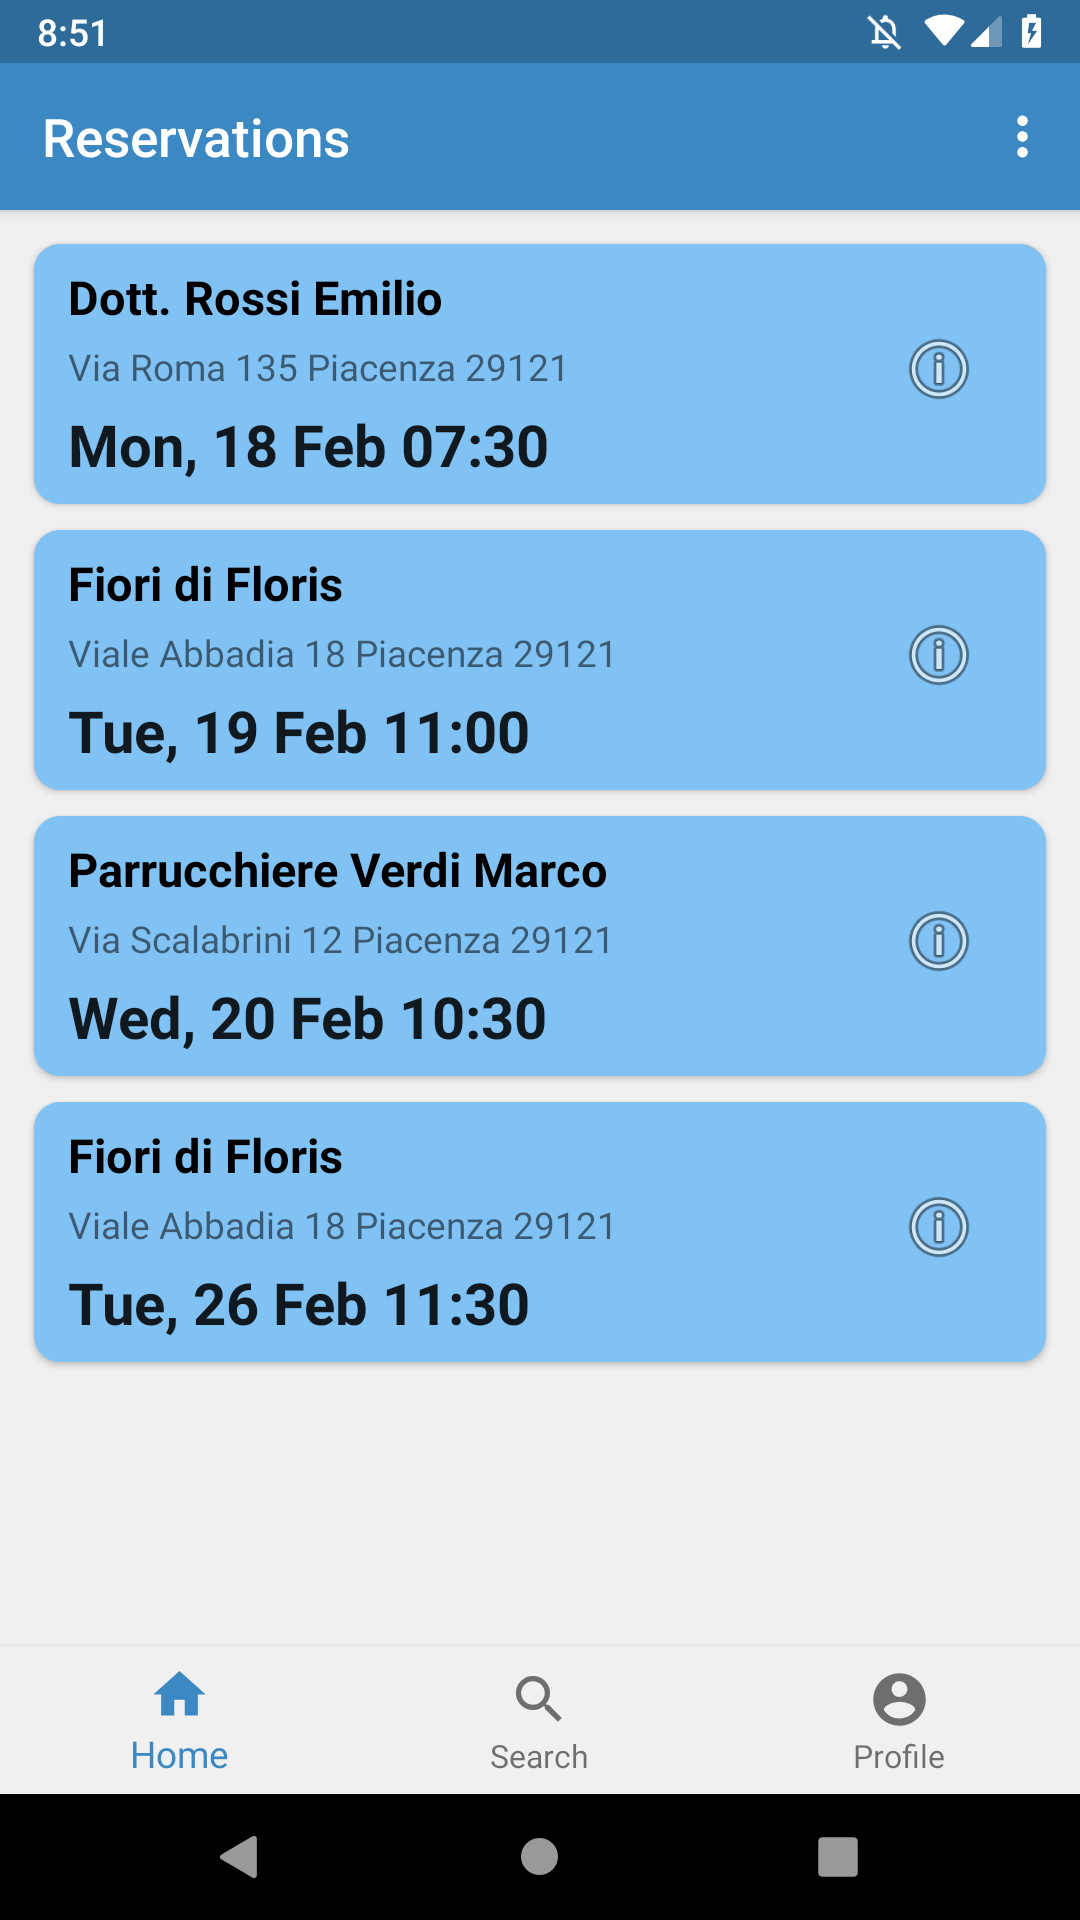
\includegraphics[height=.4\textheight, keepaspectratio=true]{Img/Screens/Customer_Home}
  \caption{Customer's home page}
\end{subfigure}%
\begin{subfigure}{.5\textwidth}
  \centering
  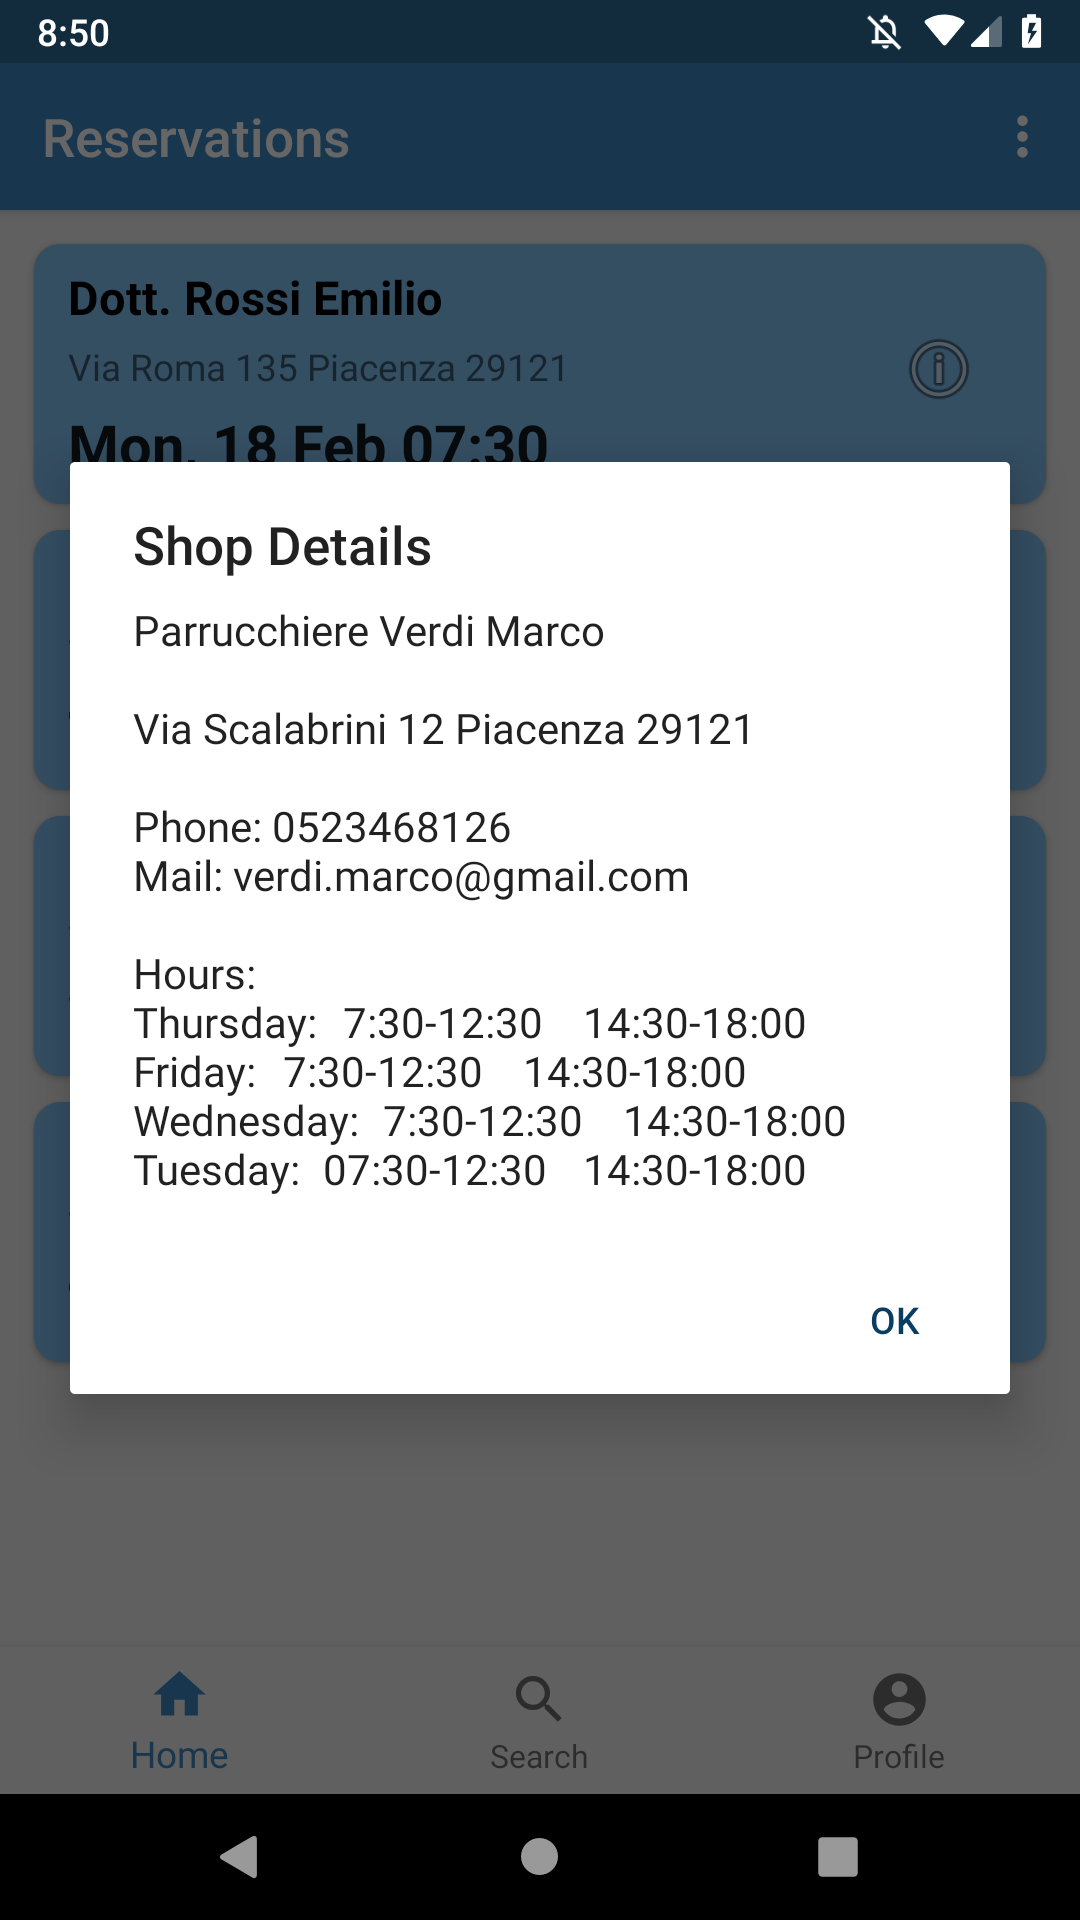
\includegraphics[height=.4\textheight, keepaspectratio=true]{Img/Screens/Customer_Home_Details}
  \caption{Details}
\end{subfigure}
\caption{Customer home page with next reservations (a) details shown when the (i) icon is pressed(b).}
\end{figure}

\begin{figure}[h]
\centering
\begin{subfigure}{.5\textwidth}
  \centering
  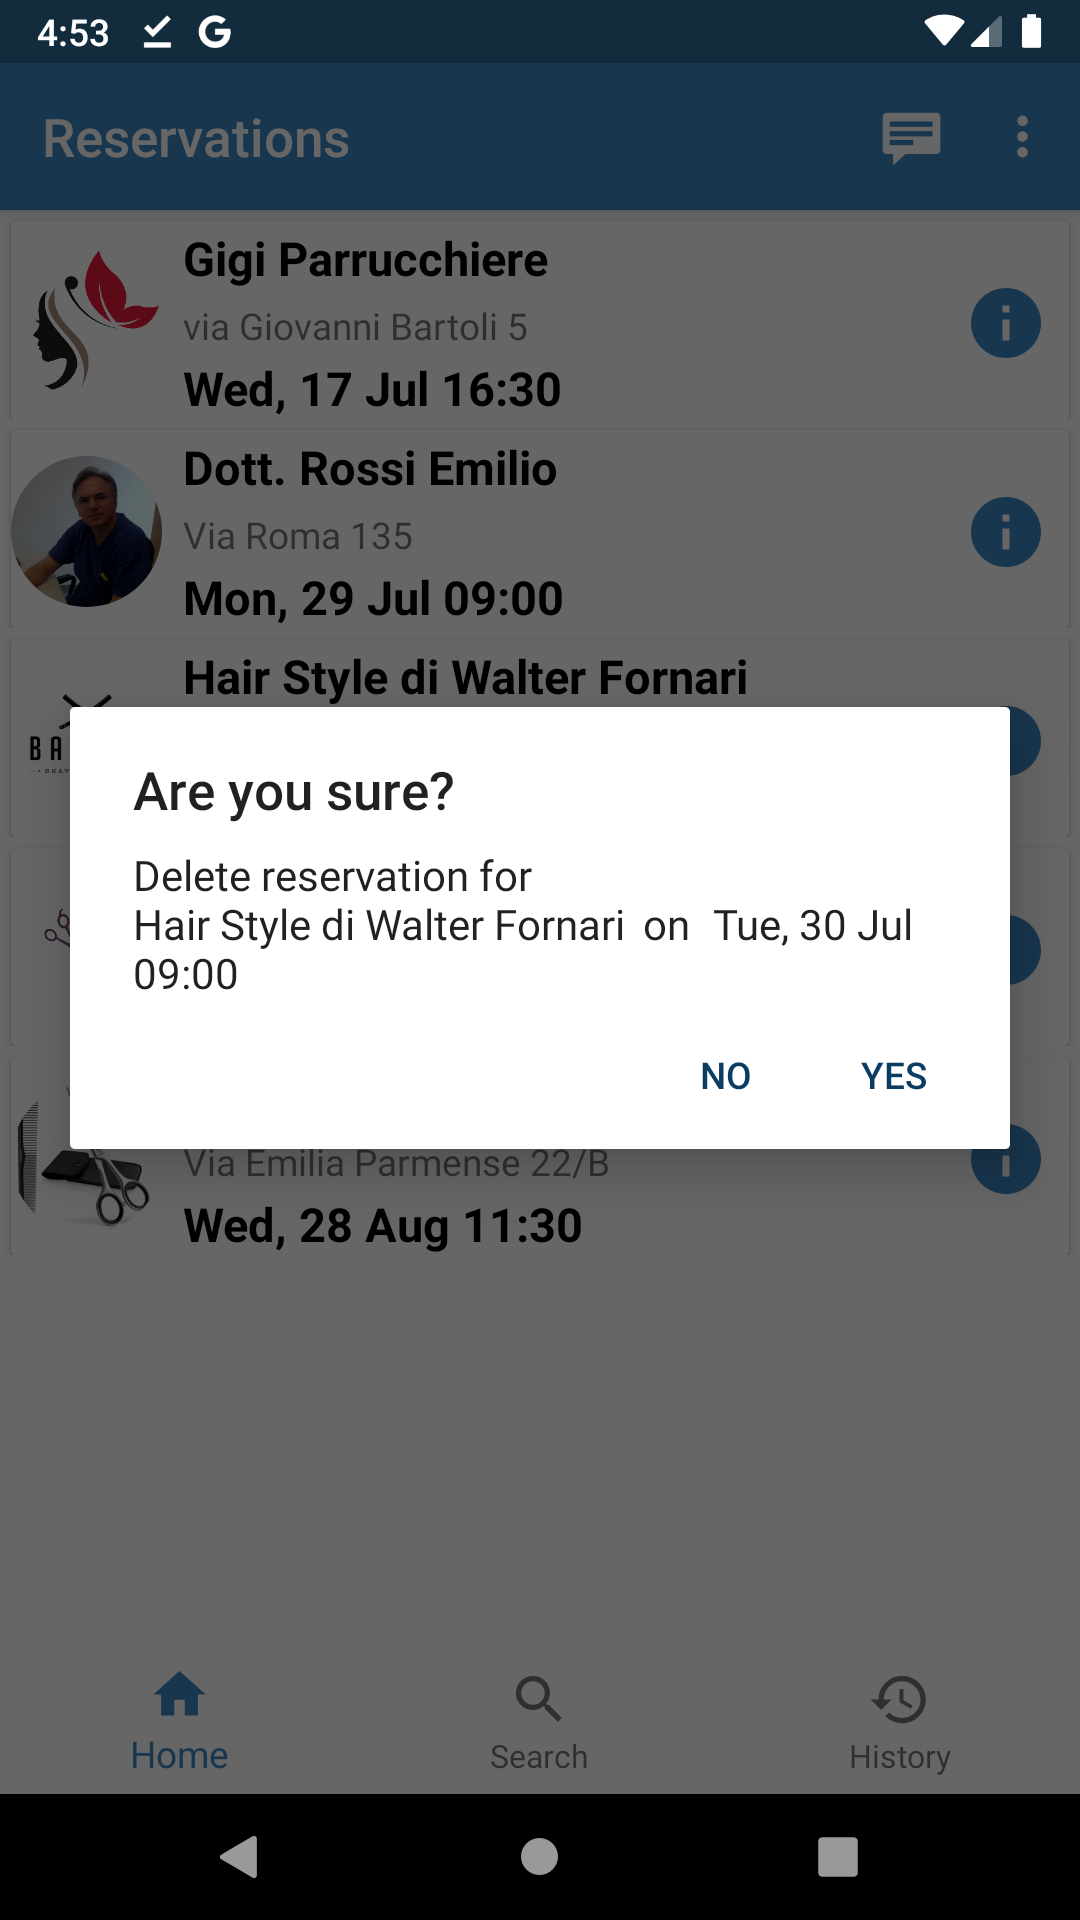
\includegraphics[height=.4\textheight, keepaspectratio=true]{Img/Screens/Customer_Home_Delete}
  \caption{Delete reservation}
\end{subfigure}%
\begin{subfigure}{.5\textwidth}
  \centering
  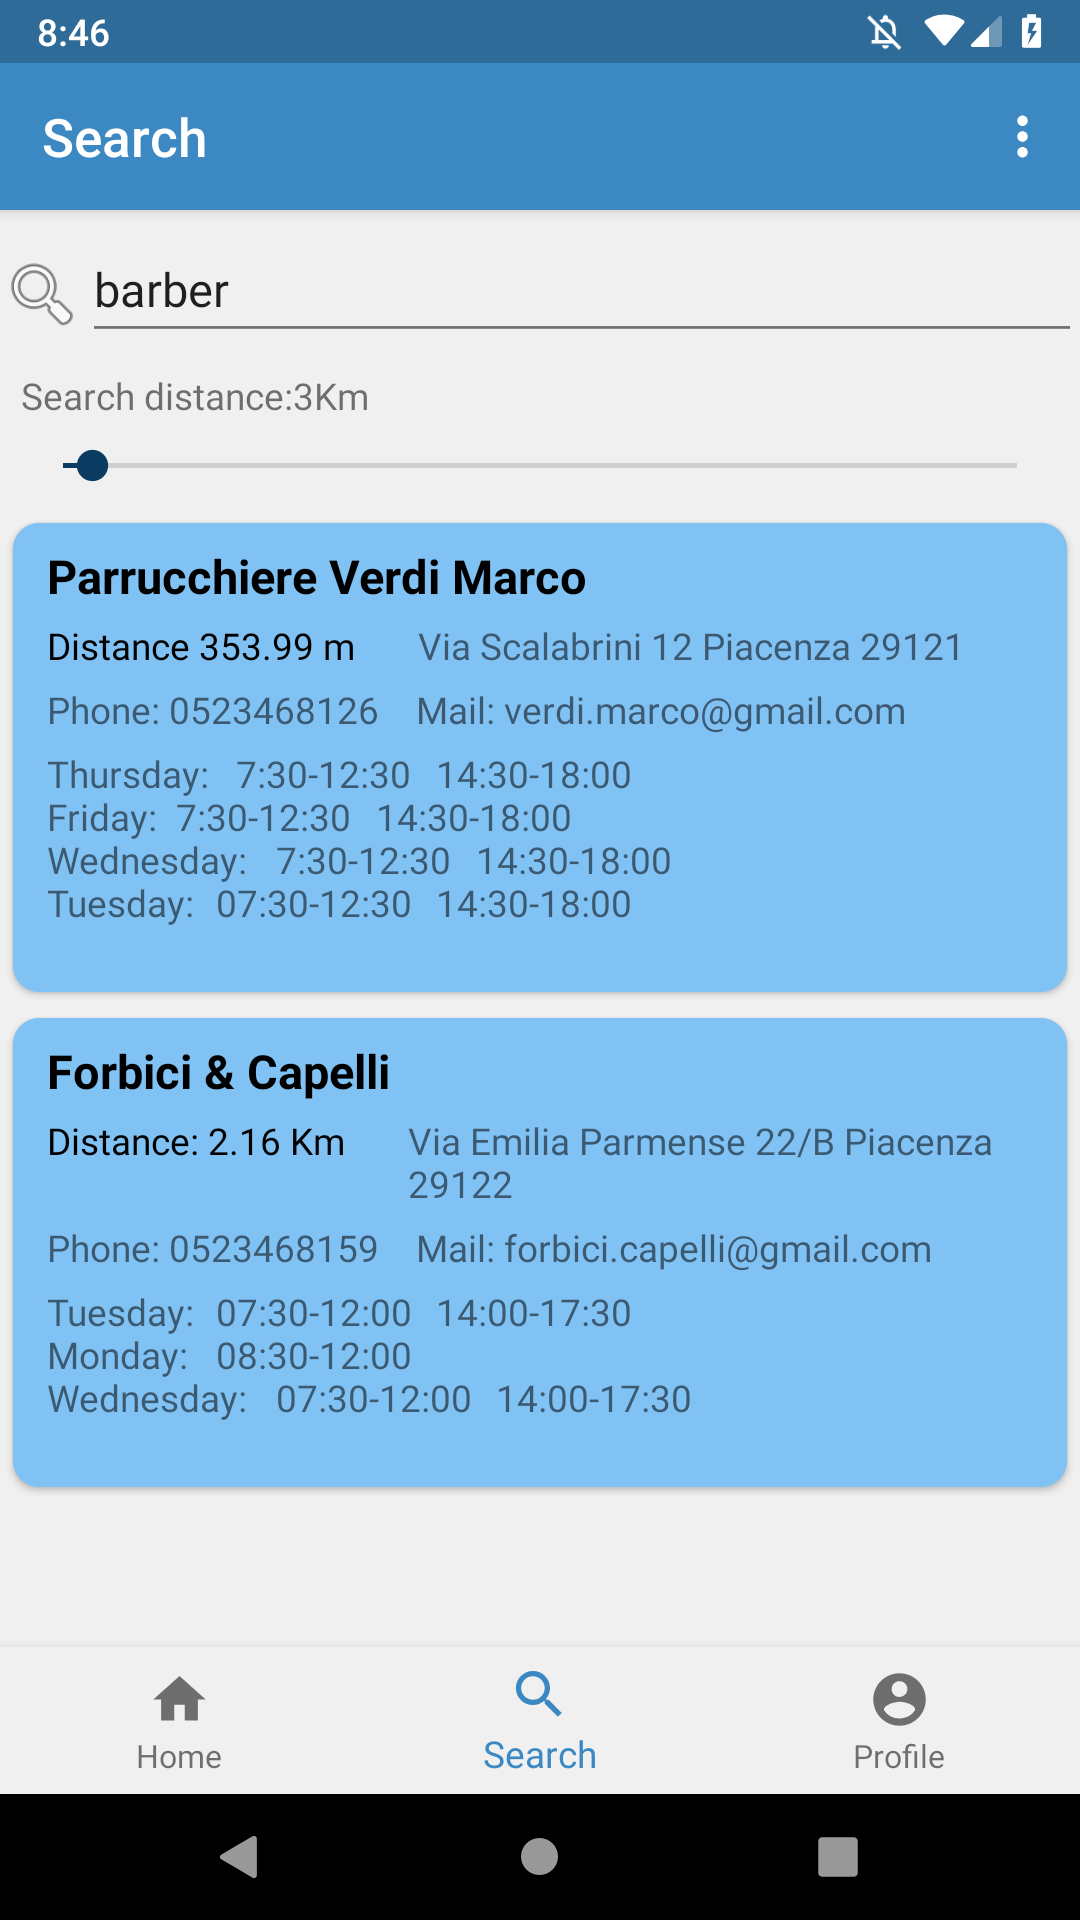
\includegraphics[height=.4\textheight, keepaspectratio=true]{Img/Screens/Customer_Search}
  \caption{Search shop}
\end{subfigure}
\caption{Popup after long click on a reservation card (a) and search page with results(b).}
\end{figure}

\begin{figure}[h]
\centering
\begin{subfigure}{.5\textwidth}
  \centering
  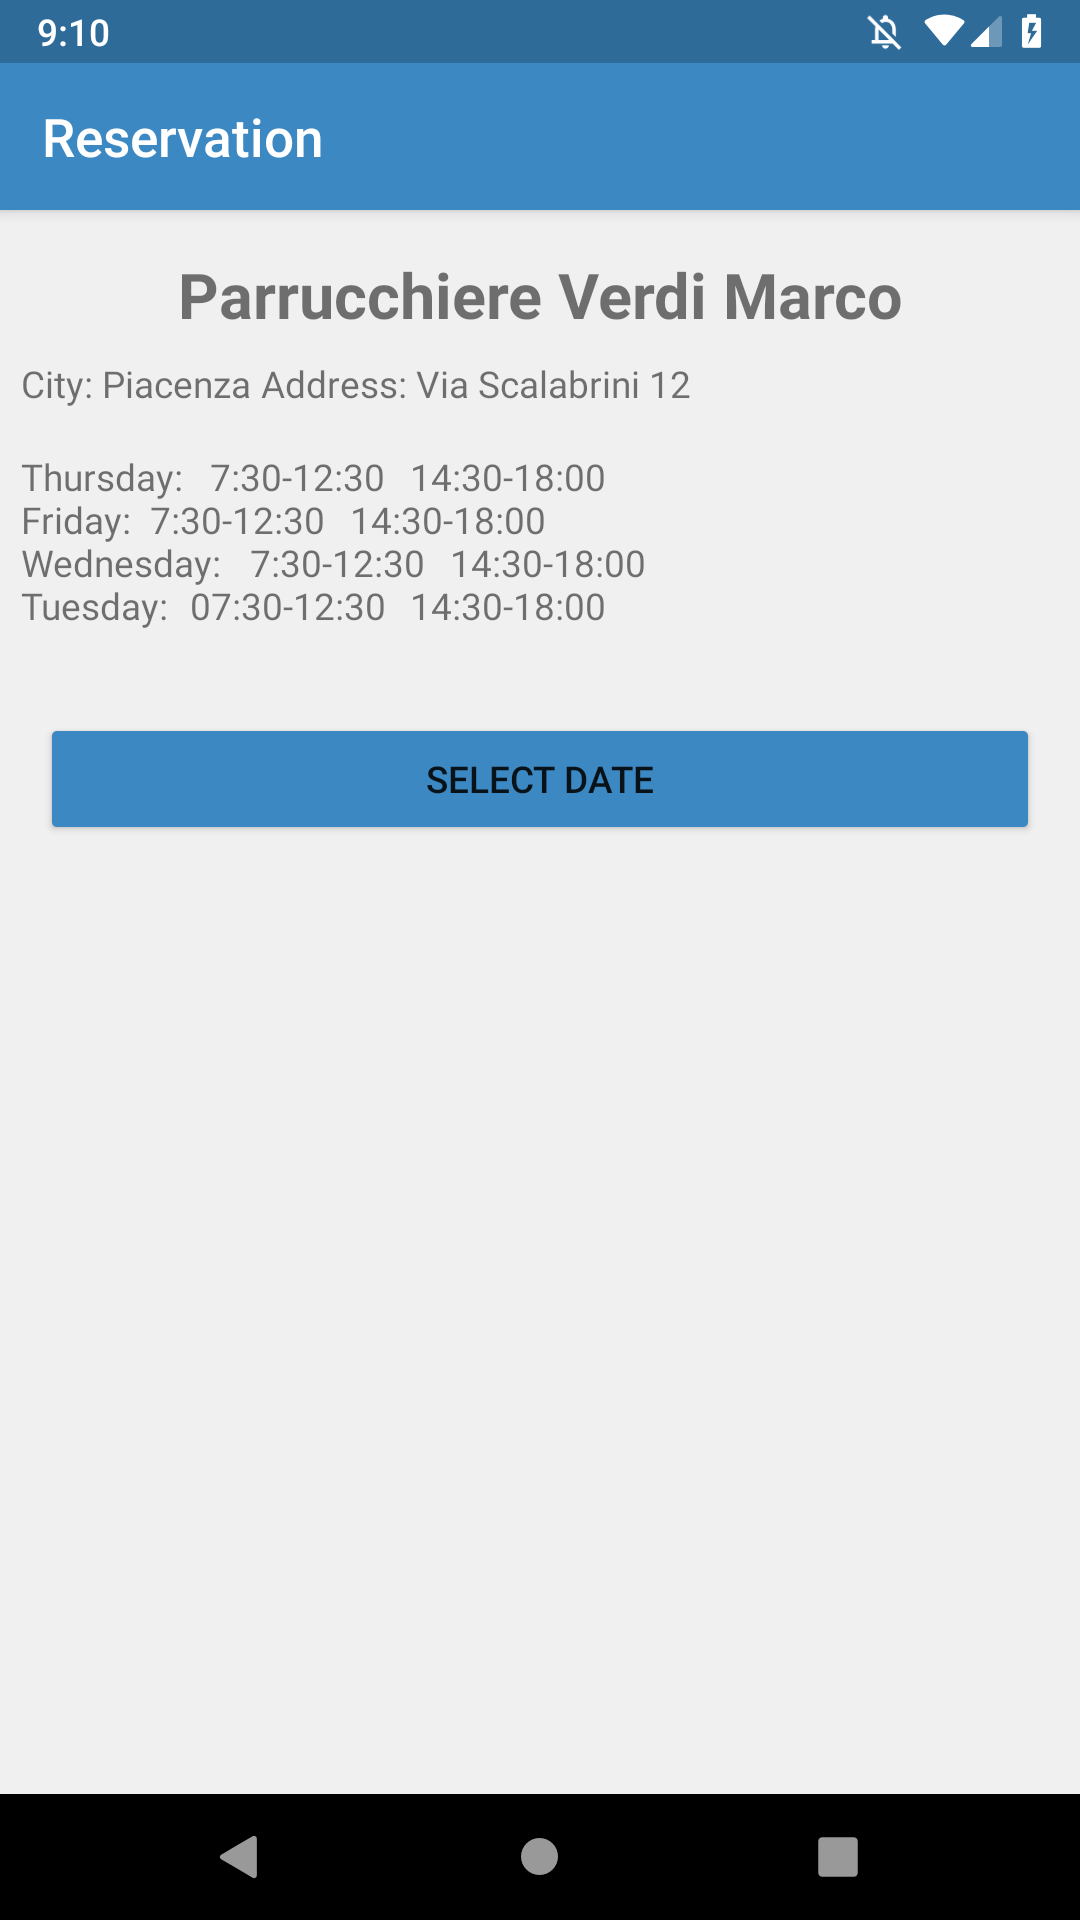
\includegraphics[height=.4\textheight, keepaspectratio=true]{Img/Screens/Customer_Search_Selected}
  \caption{Search result selection}
\end{subfigure}%
\begin{subfigure}{.5\textwidth}
  \centering
  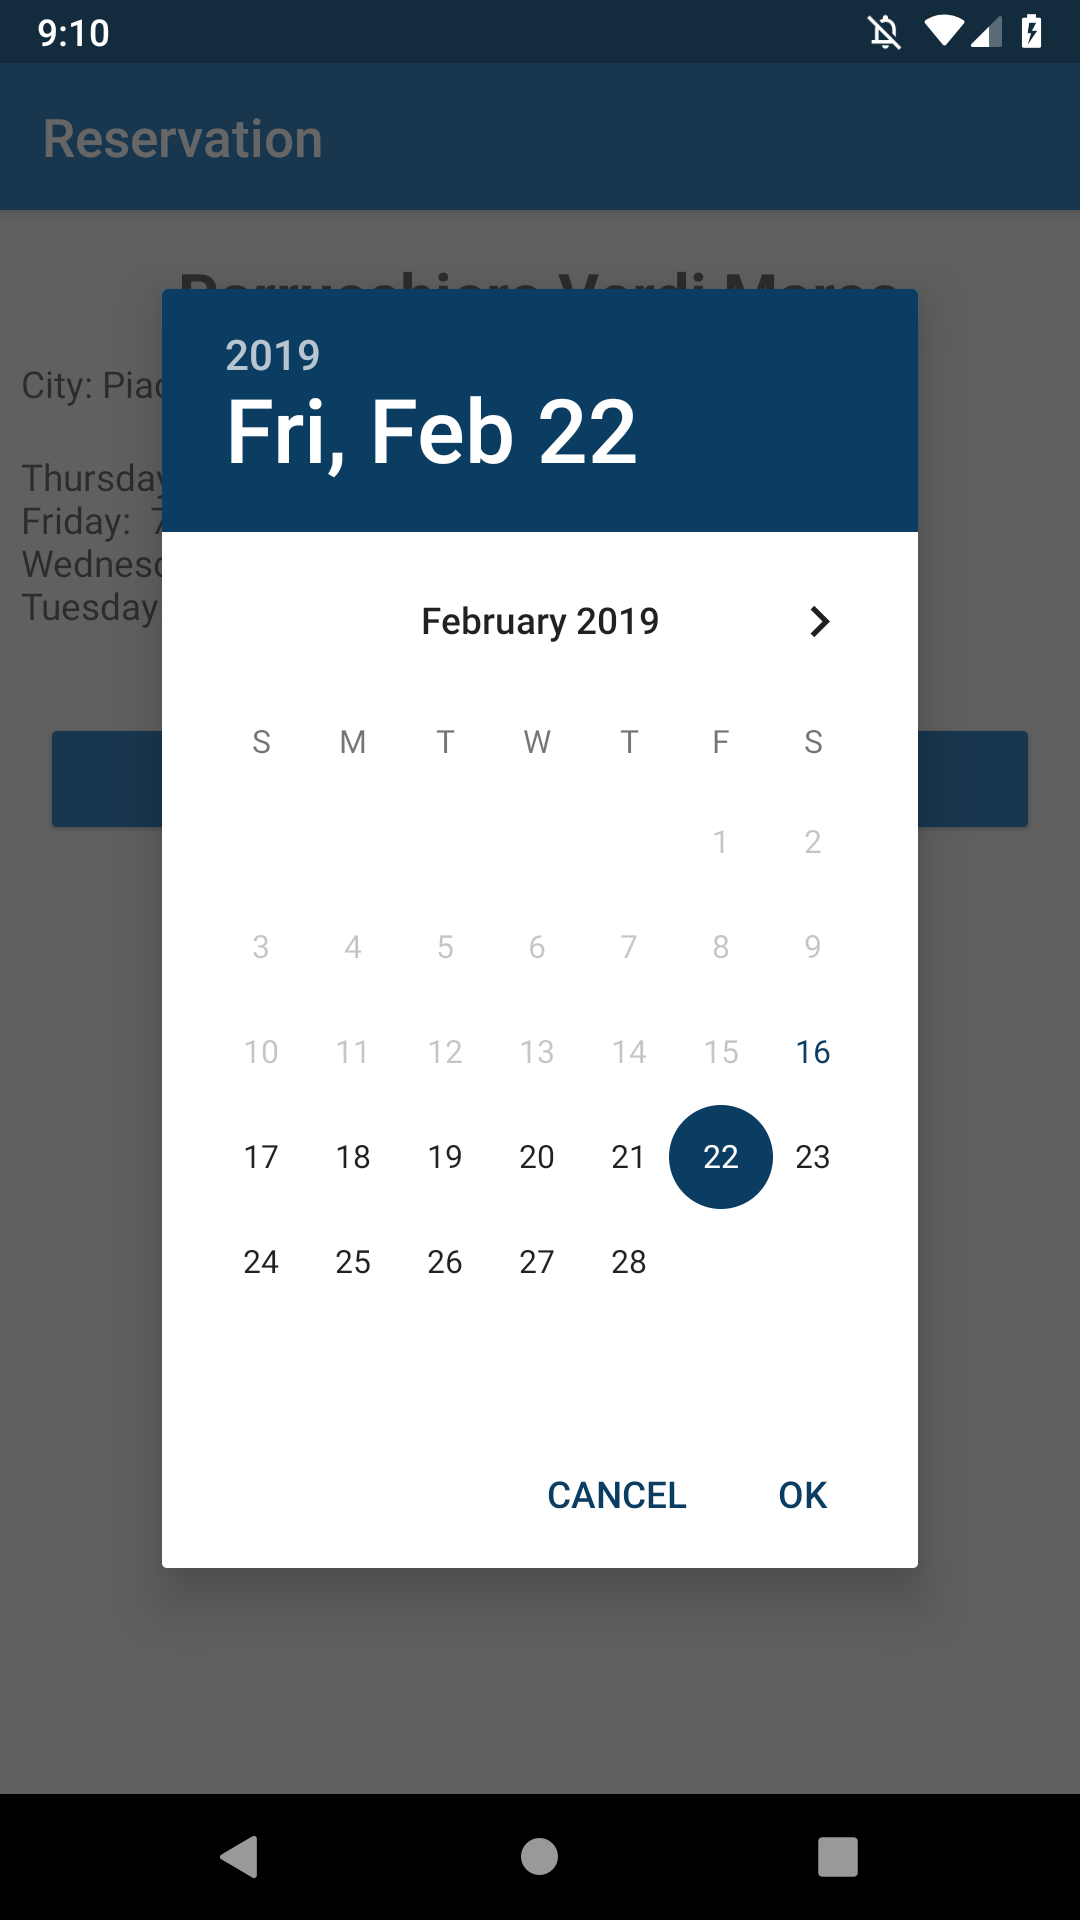
\includegraphics[height=.4\textheight, keepaspectratio=true]{Img/Screens/Customer_Search_Selected_Day}
  \caption{Picking the day}
\end{subfigure}
\caption{Page after a shop is selected (a) and day pick popup(b).}
\end{figure}

\begin{figure}[h]
\centering
  \centering
  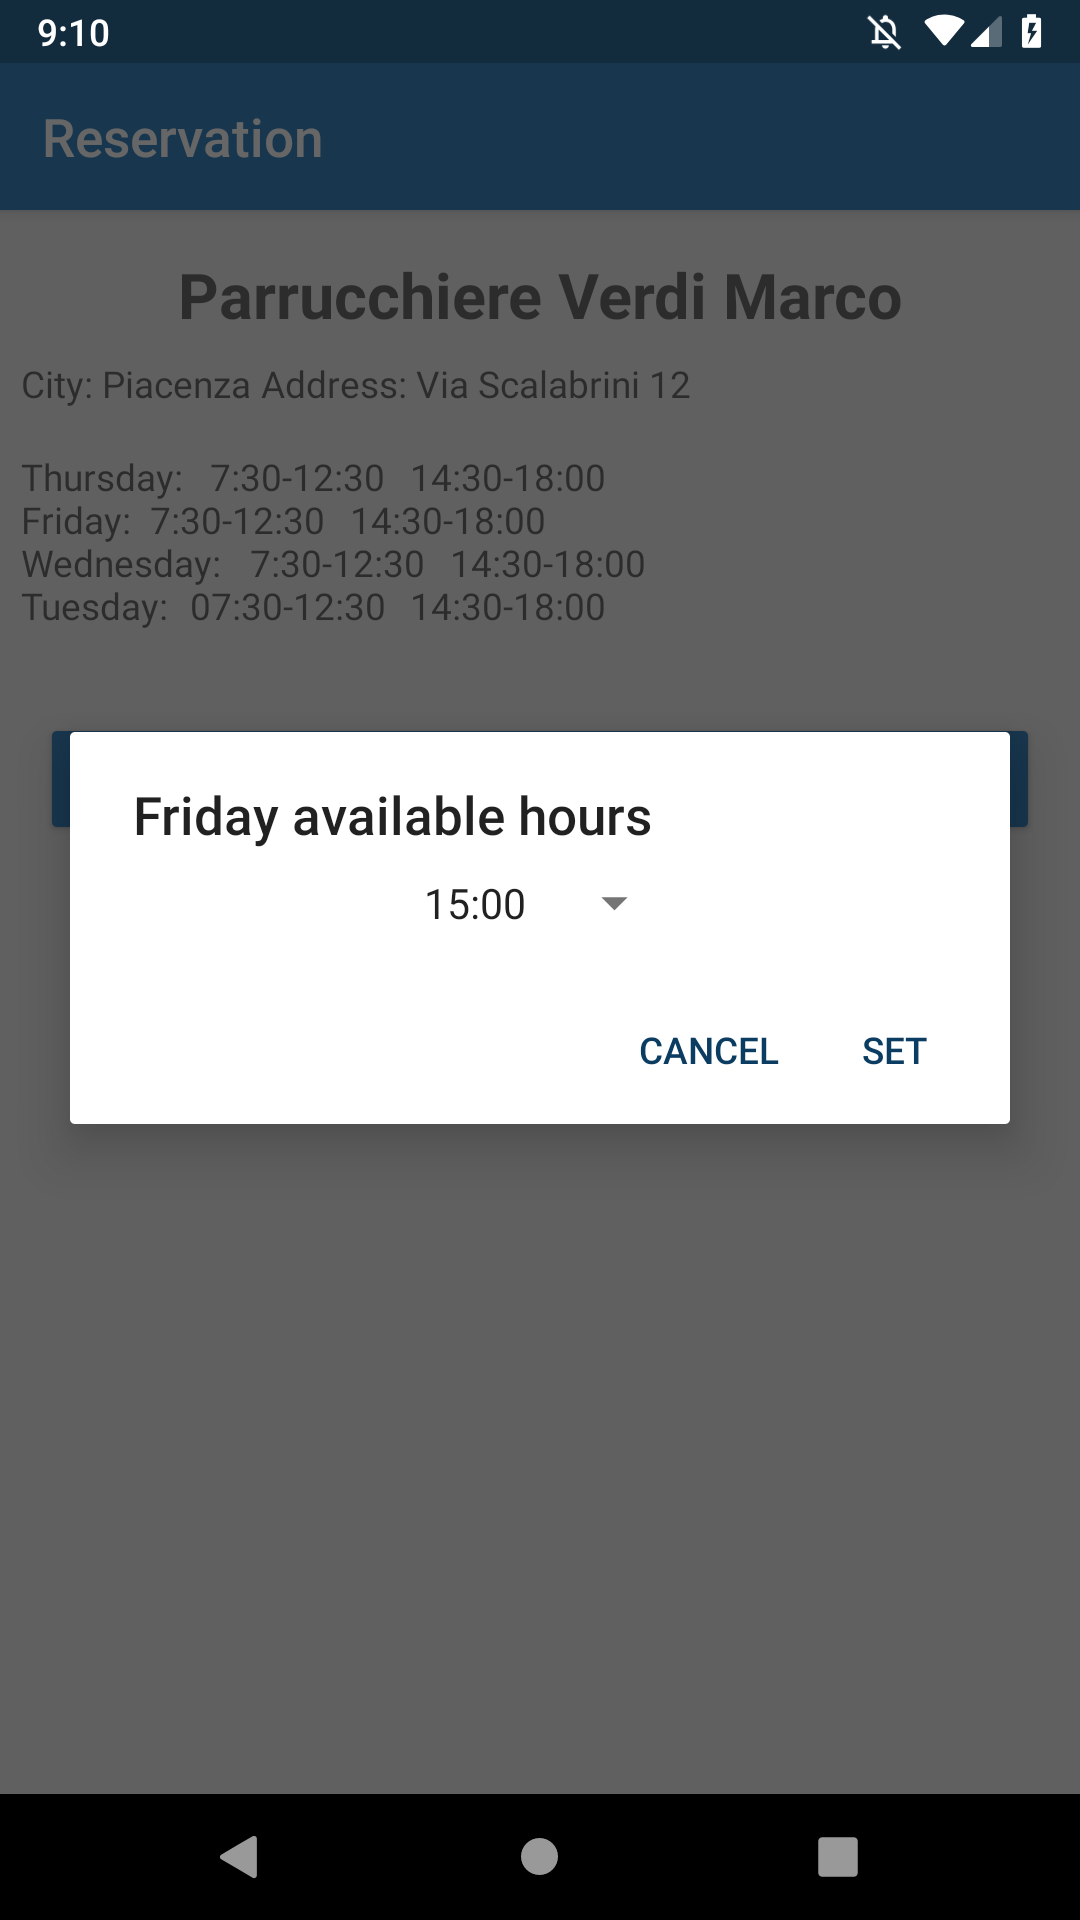
\includegraphics[height=.4\textheight, keepaspectratio=true]{Img/Screens/Customer_Search_Selected_Hour}
  \caption{Hour selection popup}
\end{figure}


